\section{Industrial applications}
\label{sec:industrial_applications}

The same argument that motivated PLC in early utility networks applies equally on the factory
floor: the communication medium is already installed. Industrial facilities are densely wired
for power delivery, and adding a data channel over this infrastructure avoids the cost and
disruption of running dedicated signal cables through walls, cable trays, and machinery
enclosures. In established plants where stopping production for days to lay new wiring is
not acceptable, this is a substantial practical advantage over both wired fieldbus extensions
and wireless systems~\cite{Pereira2015,Rinaldi2015}.

The industrial setting does, however, create conditions that are considerably harsher than
those of a domestic network. Electric motors, frequency inverters, arc-welding equipment,
and other machinery simultaneously act as impedance loads and noise sources. The resulting
disturbances---impulsive transients, frequency-dependent attenuation, and time-varying noise
across a wide spectral range---make PLC more demanding to implement than in a residential
building. The subsections that follow describe the main application areas in which PLC has
been studied and deployed in industrial and infrastructure contexts, and the measures required
to make communication reliable in these environments.

\subsection{Advanced Metering in Industrial Distribution Networks}

A practically important use of PLC in industrial facilities is energy metering across large
internal distribution networks. A factory or campus may host hundreds of power consumers, and
collecting real-time consumption data from each of them enables load monitoring, cost
allocation between production areas, and participation in demand response programs. Building
a separate wired network for this purpose is expensive; a PLC-based advanced metering
infrastructure (AMI) can instead use the low-voltage distribution cables already in place.

De~Carvalho et~al.~\cite{deCarvalho2018} examined such a system by simulating a narrowband
PLC network on a representative distribution feeder with a central substation controller.
PLC was selected because it could meet both coverage and cost constraints while reusing
existing electrical infrastructure.

Network Simulator~3 results showed that all measurement packets reached the substation within
the 2-second latency requirement for AMI, with full packet delivery over a 24-hour simulation.
The required data volume was small compared with channel capacity, leaving headroom for future
growth. Overall, the study supports PLC as a practical fit for low-rate industrial metering.

\subsection{Motor Feedback over Feeder Cables}

A more demanding application involves using the cable that carries power to an electric
motor also as the return path for control and diagnostic data. In drive systems, real-time
information such as rotor speed, winding temperature, or vibration level is measured at
the motor and must be sent back to the inverter for closed-loop control. Conventionally
this requires a separate signalling cable alongside the power feeder, which can span
hundreds of metres and adds significant installation and maintenance effort in production
environments~\cite{Ginot2010}.

Using the feeder cable itself as the communication medium eliminates the need for this
additional wiring. A PLC modem at the motor modulates a data signal onto the cable; a
second modem at the inverter demodulates it (see Fig.~\ref{fig:motor_plc}). The difficulty, studied experimentally by
Ginot et~al.~\cite{Ginot2010}, is that the feeder does not carry a sinusoidal voltage
in this case: it carries the pulse-width-modulated (PWM) output of the inverter, with
switching transients whose amplitude is proportional to the DC bus voltage.

\begin{figure}[h]
    \centering
    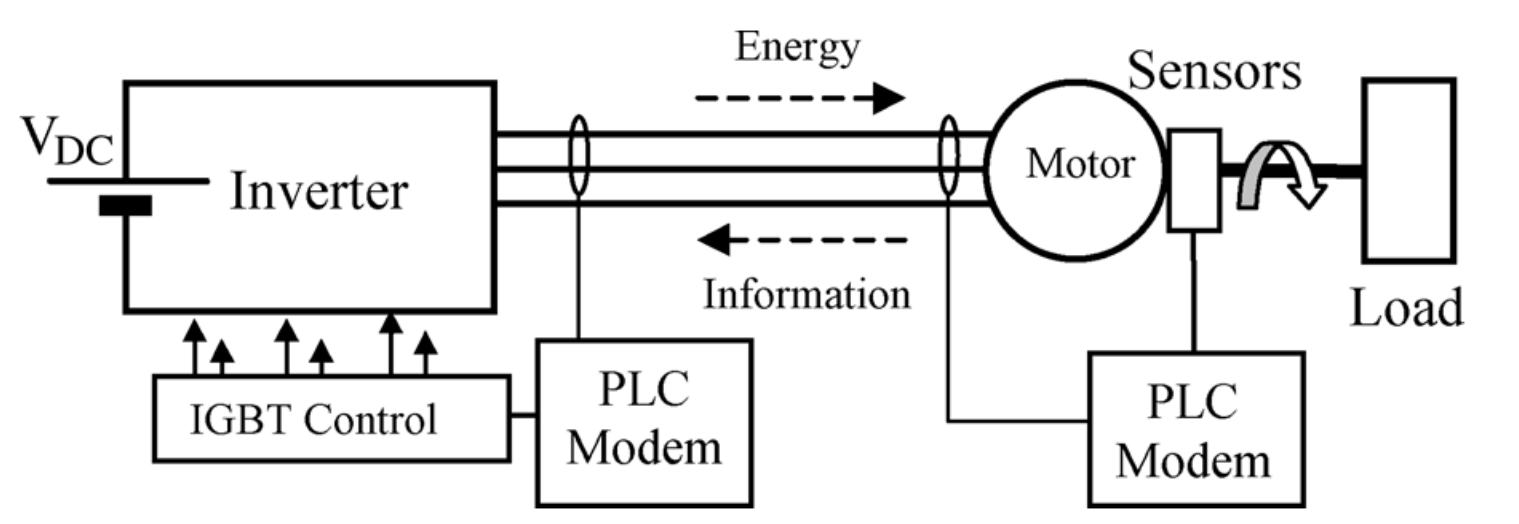
\includegraphics[width=\columnwidth]{assets/motor-feedback-loop}
    \caption{PLC-based motor feedback loop after~\cite{Ginot2010}. The communication signal
    shares the feeder cable with the PWM power waveform.}
    \label{fig:motor_plc}
\end{figure}

Tests demonstrated that throughput degraded sharply as the DC bus voltage increased,
and communication failed entirely above 100\,V without additional measures. The root
cause was switching noise from the inverter falling into the communication band. Inserting
an LCL passive filter at the inverter output reduced these
transients and restored reliable communication up to practical drive voltages. The principal
engineering lesson is that cable attenuation is usually manageable; inverter noise is the
dominant limiting factor.

\subsection{Railway Signalling and Infrastructure Control}

Metro railway systems present a different use case in which PLC, combined with supervisory
control, offers advantages over conventional communication-based train control. Train
operation requires real-time exchange of position, speed, and safety data between trains,
stations, and a central operations centre. Radio-based communication systems used for
this purpose are effective under normal conditions, but their performance can deteriorate
under congestion or if the wireless link is disrupted, and they typically depend on a
continuous upstream connection for full functionality.

Tomar et~al.~\cite{Tomar2023} proposed a metro-rail control architecture that combines
Power Line Communication links over the traction power infrastructure with a central
SCADA layer for monitoring and operator supervision. In their design, station-side
controllers perform local train tracking and safety functions, while status information is
forwarded to the
Operational Control Centre. A key reliability requirement was that core tracking and
emergency functions remain available even when the traction supply is interrupted---a
condition in which radio-dependent systems may lose their communication path. The study
reports that this local control capability, together with PLC-based backhaul and central
supervision, helped preserve service continuity under fault conditions.

Compared with the conventional Communication-Based Train Control architecture, the
proposed arrangement improved position-reporting consistency and reduced false alarms,
with faster recovery after interruptions and clearer central operator supervision.

\subsection{Channel Conditions and Protocol Selection in Practice}

The performance achievable in any given installation depends heavily on the electrical
environment at that site, and choosing the right frequency band is often more important
than the choice of coding or modulation scheme. Rinaldi et~al.~\cite{Rinaldi2015} built
a multi-protocol PLC analyser around a software-defined radio architecture and deployed
it in a real truck manufacturing plant to characterise the low-voltage channel. Their
measurements showed that error rates worsened strongly over longer cable runs, and that
the lower-frequency region was most affected by machinery noise. In this setting, operation
below 100\,kHz was not recommended.


Pereira et~al.~\cite{Pereira2015} tested G3-PLC modems across multiple frequency bands
and subcarrier modulations in a laboratory fitted with six three-phase induction motors
and a frequency inverter. The inverter was the dominant disturbance source: performance
in lower-frequency CENELEC-A conditions degraded strongly, while higher-frequency FCC-band
operation was markedly more reliable.

ROBO (Robust Operation) mode, defined within the G3-PLC standard, addresses the noise
problem by adding strong redundancy, trading throughput for robustness under heavy noise.
For low-rate tasks such as metering and status reporting, robust modes in higher bands are
often the most practical option. Where only lower bands are available, on-site channel
characterisation remains essential because noise conditions are highly plant-specific.

The general picture that emerges from these studies is that PLC in industry is not a
plug-and-play technology. Careful frequency selection, appropriate modulation robustness,
and---where motor drives are involved---output filtering are prerequisites. Within those
constraints, PLC provides a communication path over infrastructure that already exists,
at a cost that dedicated cabling or wireless repeater networks cannot match.